\documentclass[../../main.tex]{subfiles}
\begin{document}
	\section{Introduction}
		Oldschool Runescape is a MMORPG which features combat. In combat, players are awarded experience for damage dealt to their opponents (often called monsters). The mechanics of combat involve accuracy, maximum damage, attack speed, among other details. There have been several attempts to quantify the experience rates according to a player's, and their opponent's levels and equipment. Although they are quite accurate, there are additional corrections that can be applied. Additionally extensions to more complex fighting scenarios has not been performed. We will be specifically considering applications to the Nightmare Zone, a common method of training combat. This game is played with long term investments and considerations in mind, as many achievements are achieved over periods of months or even years. In this sense, even minor optimizations can result in real-world savings for the player. Furthermore, a codebase accompanies this article which allows for more advanced use of the derived formulas (such as in optimization problems). These are the central motivations for this study (and its fun!).

	\section{Damage}
		The \href{https://oldschool.runescape.wiki/w/Maximum_hit}{official Wiki page} provides a very good review of maximum hit mechanics. For completion we will provide a brief summary. For some reason, it does not contain information about accuracy calculations. These are can be found (unofficially) from \href{https://www.osrsbox.com/blog/2019/01/22/calculating-melee-dps-in-osrs/}{osrsbox} (which references \href{https://docs.google.com/spreadsheets/d/1wzy1VxNWEAAc0FQyDAdpiFggAfn5U6RGPp2CisAHZW8/edit#gid=158500257}{DPS calculator by Bitterkoekje} the \href{https://web.archive.org/web/20190905124128/http://webcache.googleusercontent.com/search?q=cache:http://services.runescape.com/m=forum/forums.ws?317,318,712,65587452}{forum post} of which has been archived), \href{https://www.reddit.com/r/2007scape/comments/40bvk6/accuracy_and_exphr_combat_formula/}{MachOSRS} (reddit), and \href{https://www.reddit.com/r/2007scape/comments/5lrty0/math_inside_corrected_accuracy_formula/}{[deleted]} (reddit).  Following this, we will take care to accurately determine the number of hits required to kill an opponent with novel calculations. Related calculation have been performed by \href{https://www.reddit.com/r/2007scape/comments/4d6l7j/effects_of_overkill_on_dps/}{Nukelawe}, which discusses the impact of overkill on expected damage, which is often neglected in damage calculations. We will take this further to calculating expected number of hits to kill an opponent.
		\subsection{Maximum Hit}
			$m$ will denote the player's maximum hit. Ranged and melee have a similar method for calculating the maximum hit. For these, there are 5 bonuses that a player can obtain to boost their maximum hit. These are bonuses from, potions, prayer, other, style, and special attack. These will be referred to as: $B^\text{pot}$, $B^\text{pray}$, $B^\text{other}$, $B^\text{style}$, $B^\text{SA}$, respectively. An effective damage level is defined as
			\begin{align}
				L^\text{eff} \equiv \left \lfloor \left(L + B^\text{pot} \right)B^\text{pray}B^\text{other} \right \rfloor + B^\text{style},
			\end{align}
			where $L$ is either the ranged level or strength level. The base damage, $D^\text{base}$ is then given by,
			\begin{align}
				D^\text{base} = C_0 + C_1L^\text{eff} + C_2 E^\text{str} + C_3 E^\text{str}S^\text{eff},\\
				\text{where}\,\,\, \{C\} = \left\{1.3, \frac{1}{10}, \frac{1}{80}, \frac{1}{640}\right\},
			\end{align}
			and $E^\text{str}$ is the ranged or melee strength bonus of the worn equipment. The max hit, $M$ is finally given by,
			\begin{align}
				M = \left \lfloor D^\text{base} B^\text{SA}\right \rfloor,
			\end{align}
			where $B^\text{SA} = 1$ if no special attack is being used.

 			For melee, the Keras and Saradomin Sword are exceptions this final equation. For ranged, it should be noted that bolt effects only have probabilities of activating (and therefore increasing $M$). To handle this, we can define an effective or average max hit: $\langle M \rangle = P M$, where $P$ is the probability of activation.
			\subsubsection{Magic}
				The base damage for a magic spell is given according to that spell. However multiplicative bonuses are provided by various equipment. For a single bonus is given by,
				\begin{align}
					M = D^\text{base}E^\text{str},
				\end{align}
				where now $E^\text{str}$ is the multiplicative magic damage bonus (think ``magic\\strength''). In general, these effects stack, but intermediate flooring calculations can impact the max hit. Charge, magic dark, salamanders, and trident of the seas/swamp have alternate calculations (although charge can be seen as a temporary 1.5x multiplier).
		\subsection{Accuracy}
			$A$ will denote the player's probability of a successful hit (called accuracy). This attribute depends on both the player and the opponents stats. The attacker rolls an attack role, while the defender rolls a defensive roll. First effective levels are calculated,
			\begin{align}
				L^\text{eff}_* \equiv \left \lfloor \left(L + B^\text{pot} \right)B^\text{pray}B^\text{other} \right \rfloor + B^\text{style} + 8,
			\end{align}
			where the subscript $*$ is used to denote the difference between the effective damage levels discussed above, and these effective accuracy levels.
			Then the maximum roll is given by,
			\begin{align}
				R_\text{max} = \left \lfloor L_*^\text{eff} (E + 64)\right \rfloor,
			\end{align}
			where $E$ is the equipment bonus for the respective attack or defense style.
			Now the accuracy is given according to,
			\begin{empheq}[box=\fbox]{align}
				A = \begin{cases}
					1 - \frac{1}{2}\frac{D_\text{max} + 2}{A_\text{max} + 1} & A_\text{max} \ge D_\text{max} \\
					\frac{A_\text{max}}{2D_\text{max} + 2} & \text{else},
				\end{cases}
			\end{empheq}
			where $A_\text{max}$ and $D_\text{max}$ represent the maximum attack and defense rolls ($R_\text{max}$) respectively. No information suggests magic accuracy is any different. No other work / official statements show how special attacks factor into this. It is a fair assumption that $A^\text{eff} = AB^\text{SA}$ for special attacks that increase accuracy (since all effective are multiplicative, and no flooring needs to be done for accuracy).

		\subsection{Average Damage}
			Here beings the new calculations (if the previous sections were unclear, please read the cited references). The damage done during an attack is uniformly distributed on $[0, m]$, so each integer between 0 and the max hit have an equal chance of $1/(m + 1)$ of occurring. The average damage done during an attack is the expectation,
			\begin{align}
				\langle D \rangle &= \frac{1}{m+1}\sum_{i=0}^{m} i\\
				&= \frac{1}{\cancel{m+1}}\frac{m(\cancel{m+1})}{2}\\
				&= \frac{m}{2}
			\end{align}
			However, this makes the assumption that the player can always hit up to their max hit. This is not the case if the opponent has less health, $h$ than the maximum hit. This effect is sometimes referred to as \textit{overkill} damage.
			\begin{center}
			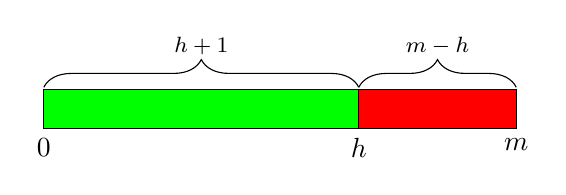
\begin{tikzpicture}
				\filldraw[fill=green, draw=black] (0,0) node[anchor=north] {$0$} -- (4,0) node[anchor=north] {$h$} -- (4,0.5) -- (0,0.5) -- (0,0);
				\filldraw[fill=red, draw=black] (4,0) -- (6,0) node[anchor=north] {$m$} -- (6,0.5) -- (4,0.5) -- (4,0);
				\draw [decorate,decoration={brace,amplitude=10pt},xshift=0pt,yshift=15pt]
				(0,0) -- (4,0) node [black,midway,yshift=15pt]{
					\footnotesize $h+1$
				};
				\draw [decorate,decoration={brace,amplitude=10pt},xshift=0pt,yshift=15pt]
				(4,0) -- (6,0) node [black,midway,yshift=15pt]{
					\footnotesize $m-h$
				};
			\end{tikzpicture}
			\end{center}
			In this case, we could hit every integer below $h$ each with a probability of $1/(m+1)$, and we could hit exactly $h$ with a probability of $(m-h)/(m+1)$,
			\begin{align}
				\langle D \rangle_{h < m} &= \frac{1}{m+1}\sum_{i=0}^{h} i + \frac{m-h}{m+1}h \\
				&= \frac{1}{m+1}\frac{h(h+1)}{2} + \frac{m-h}{m+1}h \\
				&= \frac{h}{2}\frac{2m-h+1}{m+1}\\
				&= \frac{h}{2}\left(1 + \frac{m - h}{m+1}\right)\\
				&= \frac{h}{2}\left(2 - \frac{h + 1}{m+1}\right)
				% &= \frac{h^2}{2m} + \frac{h}{2m} + h - \frac{h^2}{m} \\
				% &= -\frac{h^2}{2m} + \left(\frac{1}{2m} + 1\right)h \\
			\end{align}

			Overall then, our expected damage on a successful hit is
			\begin{align}
				\boxed{
					\langle D \rangle = \frac{1}{2}\begin{cases}
						m &\text{if $h \ge m$} \\
						h\left(2 - \frac{h + 1}{m+1}\right) &\text{if $h < m$} \\
					\end{cases}
				}
			\end{align}
		\subsection{Health after $n$ Attacks}
			To determine the health of an opponent after a given number of \textit{successful!} attacks (we can include accuracy after), we note that the above gives us a recursive function for the health, $h_n$ of an opponent after $n$ attacks,
			\begin{align}
				h_{n+1} = h_{n} - \frac{1}{2}\begin{cases}
					m &\text{if $h_n \ge m$} \\
					h_n\left(2 - \frac{h_n + 1}{m+1}\right) &\text{if $h_n < m$}.
				\end{cases}
			\end{align}
			This however is unwieldly. Instead we consider it in two parts. While $h$ is above or equal to $m$ we the solution to the above becomes,
			\begin{align}
				h_{n+1} &= h_{n} - \frac{m}{2} \\
				&\implies h_n = h_0 - n\frac{m}{2},\label{eq:h_crude}
			\end{align}
			where $h_0$ is the maximum / starting health. The solution to the other is a bit more complex. After a certain number of iterations the health will drop below $m$ and the second case above will kick in. We'll say this occurs after $L$ iterations (noting that this \emph{average} quantity can be a non-integer),
			\begin{align}
				m &> h_0 - L\frac{m}{2} \\
				\frac{2}{m}(h_0 - m) &< L \\
				\implies L &= 2\left(\frac{h_0}{m} - 1\right).
			\end{align}
			So the expected health that the second condition starts at is given by,
			\begin{align}
				\langle h_L \rangle &= h_0 - 2\left(\frac{h_0}{m} - 1\right) \frac{m}{2}\\
				&= m.
			\end{align}
			Thus the second case is expected to starts on iteration $L$ with an initial health of $m$. For simplicity, we will define $m\equiv n-L$. Returning to our recursive function,
			\begin{align}
				h_{m+1} &= h_{m} - \frac{h_m}{2}\left(2 - \frac{h_m + 1}{m+1}\right) \\
				&= h_{m} - h_m + \frac{h_m}{2}\frac{h_m + 1}{m+1} \\
				&= \frac{h_m^2 + h_m}{2(m+1)} \\
				h_{m+1} &= \gamma (h_m^2 + h_m),\,\,\,h_0 = m, \label{eq:recur}
			\end{align}
			where $\gamma\equiv1 / 2(m+1)$. This type of recurrence relation is called a quadratic map, and unfortunately it has no closed form solution in general. Some work is shown in the appendix to attempt to simplify it, but no final form was realized. For the sake of completeness, we will call the solution to Eq.~\ref{eq:recur} $f(m; f_0)$. At this point we're left with,
			\begin{align}
					h(n; h_0, m) &=  \begin{cases}
					h_0 - \frac{1}{2}nm &\text{else if $n \le L$} \\
					f(n - L; m) &\text{otherwise}.
				\end{cases}
			\end{align}
			In general, we are more interested in the number of iterations that is required to kill an opponent which is the inverse of this function, $n=h^{-1}(h; h_0, m)$. However, since the recurrence relation cannot be solved analytically, we cannot obtain a general expression for this. We could numerically compute this result. However remember that we are dealing with \emph{expectation values} or averages. This means it is totally possible for the inverted function to say ``The opponents health will be 18 in 4.5 iterations, on average''. This is a problem because our recursive equation can only increment the iteration by one (and we can only start at $f_0$)! In the next section, we will look at an approximation that will allow us to handle non-integer expectations.

		\subsubsection{Approximate Solutions}
			Despite not being able to find a closed-form solution for Eq.~\ref{eq:recur}, we can look for approximate solutions. Although it's rare, there are a few quadratic recurrence relations that \textbf{do} have solutions. There are two relevant cases, one where a constant term is introduced, or ones where the linear term is removed. Since increasing $n$ (and therefore iterations) results in smaller and smaller $h_n$, it suggests that adding constant terms will heavily skew the results in this region. Removing the linear term is still not ideal since its contribution increases relative to the quadratic term, in the low $h_n$ limit. However this should be less significant. In this case, our recursive relation becomes,
			\begin{align}
				h_{m+1} = \gamma h_m^2.
			\end{align}
			Starting with $h_0 = m$, and looking at a few terms reveals,
			\begin{align}
				h_{1} &= \gamma^1 m^2\\
				h_{2} &= \gamma^1 h_1^2\\
					&= \gamma^1 \gamma^2 m^{(2\cdot2)}\\
				h_{3} &= \gamma^1 h_2^2\\
					&= \gamma^1 \gamma^2 \gamma^4 m^{(2\cdot2\cdot2)}\\
				\implies h_m &= \gamma^{\sum_{i=0}^{m-1} 2^i} m^{2^m}\\
							&= \gamma^{2^m-1} m^{2^m}\\
							&= \frac{1}{\gamma}(\gamma m)^{2^m}\\
						\Aboxed{h_m &= \frac{1}{\gamma}\left(\frac{1}{2} - \gamma\right)^{2^m}}
			\end{align}
			This equation is not only a closed form expression, but it can also be inverted!
			\begin{align}
				\log_2(\log_{\frac{1}{2} - \gamma} (\gamma h_m)) &= m.
			\end{align}
			This equation asymptotically reaches 0, but the opponent dying occurs when $h_m$ drops below 1 yielding an average kill on iteration,
			\begin{align}
				\log_2(\log_{\frac{1}{2} - \gamma} (\gamma)) &= m.
			\end{align}

			How can we make use of this approximation to improve our more accurate calculation? Remember that we are trying to solve the issue of non-integer iterations. Instead of beginning on iteration 0 for the iterative procedure, we can start $m$ at any real number in (0, 1), and iterate upwards on that. For example to get the health at iteration 4.87, we could use our analytic approximation to calculate 0.87 (okay - sacrifice one approximation), then iterate 4 times using the correct equation to get to the final result. So this defines our new best approximation,


			\begin{empheq}[box=\fbox]{align}\label{eq:recursive_h}
					h(n; h_0, m) &=  \begin{cases}
					h_0 - \frac{1}{2}nm &\text{if $n \le L$} \\
					\frac{1}{\gamma}\left(\frac{1}{2} - \gamma\right)^{2^{n-L}} &\text{if $n - L < 1$}\\
					f\left(n - L; \frac{1}{\gamma}\left(\frac{1}{2} - \gamma\right)^{2^{n-L}}\right) &\text{otherwise}\\
				\end{cases}\\
				\text{where, }\gamma = &\frac{1}{2(m+1)}\text{ and } L = 2\left(\frac{h_0}{m} - 1\right).\nonumber
			\end{empheq}
			To solve for when the opponents health drops below one, $n=h^{-1}(1)$, we must use a numerical root finding algorithm to solve for the zero of $|1 - h(n)|$.


			\subsubsection{Comparisons}
				We have seen several methods for calculating expected kill iterations. We can now compare all these models to the ``true'' simulated calculation. Thankfully, the final iteration only depends on the initial health and max hit. Both of these are integers, so this can easily be tabulated since both of these are capped in the game (this is not the case when accuracy is factored in). Fig.~(\ref{fig:comparison}) shows a comparison between the different methods for the number of successful hits required. In general, as the initial health becomes significantly greater the number of turns grows rapidly (as expected). The error from the simulation is largest for large max hits and low initial healths. The crude calculation has an unbounded error, whilst the recursive method is (empirically) bounded by the crude error, and has a global maximum. This justifies the recursive method as being more accurate. This is expected to improve accuracy by about 1-5\% depending on the fighters (remember that this scales over periods of weeks \& months!).
				% For max melee, this saves 11 hours!

				\begin{figure}
					\centering
					\begin{subfigure}{.5\textwidth}
						\centering
						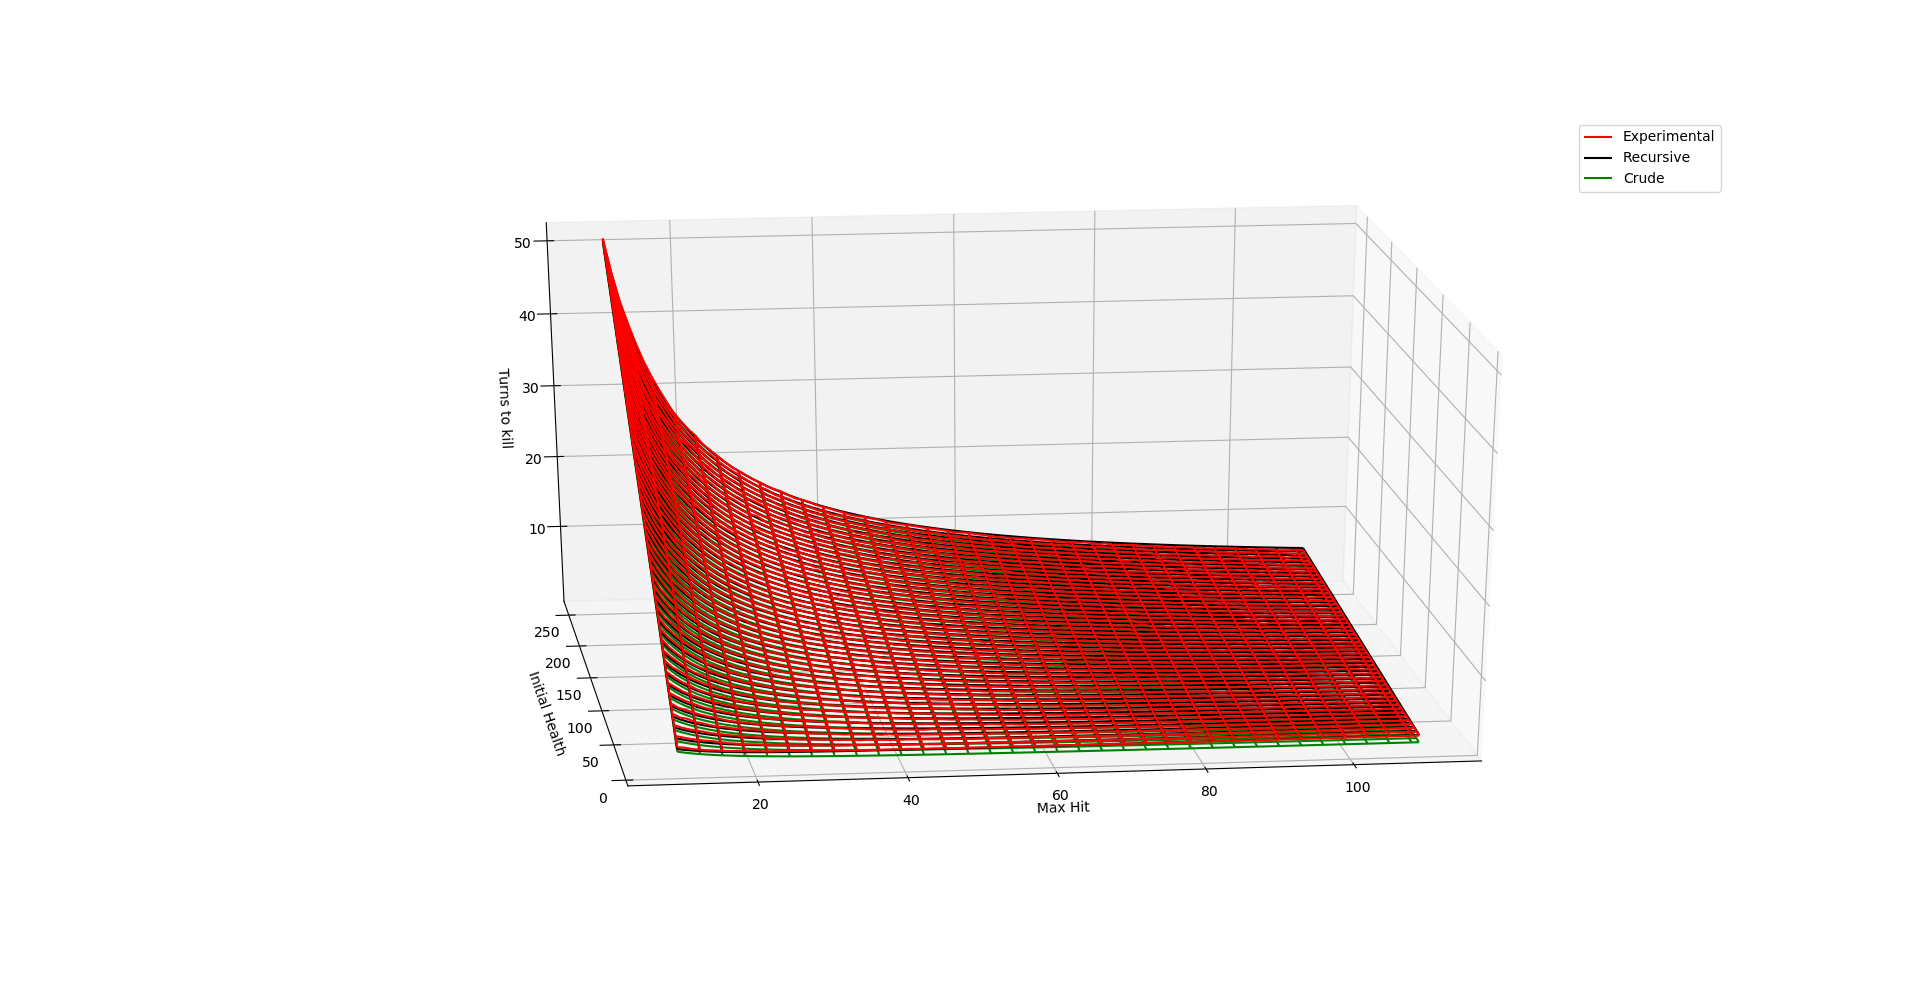
\includegraphics[width=\linewidth]{img/h2k_h2.png}
						\caption{Turns to Kill}
						% \label{fig:sub1}
					\end{subfigure}%
					\begin{subfigure}{.5\textwidth}
						\centering
						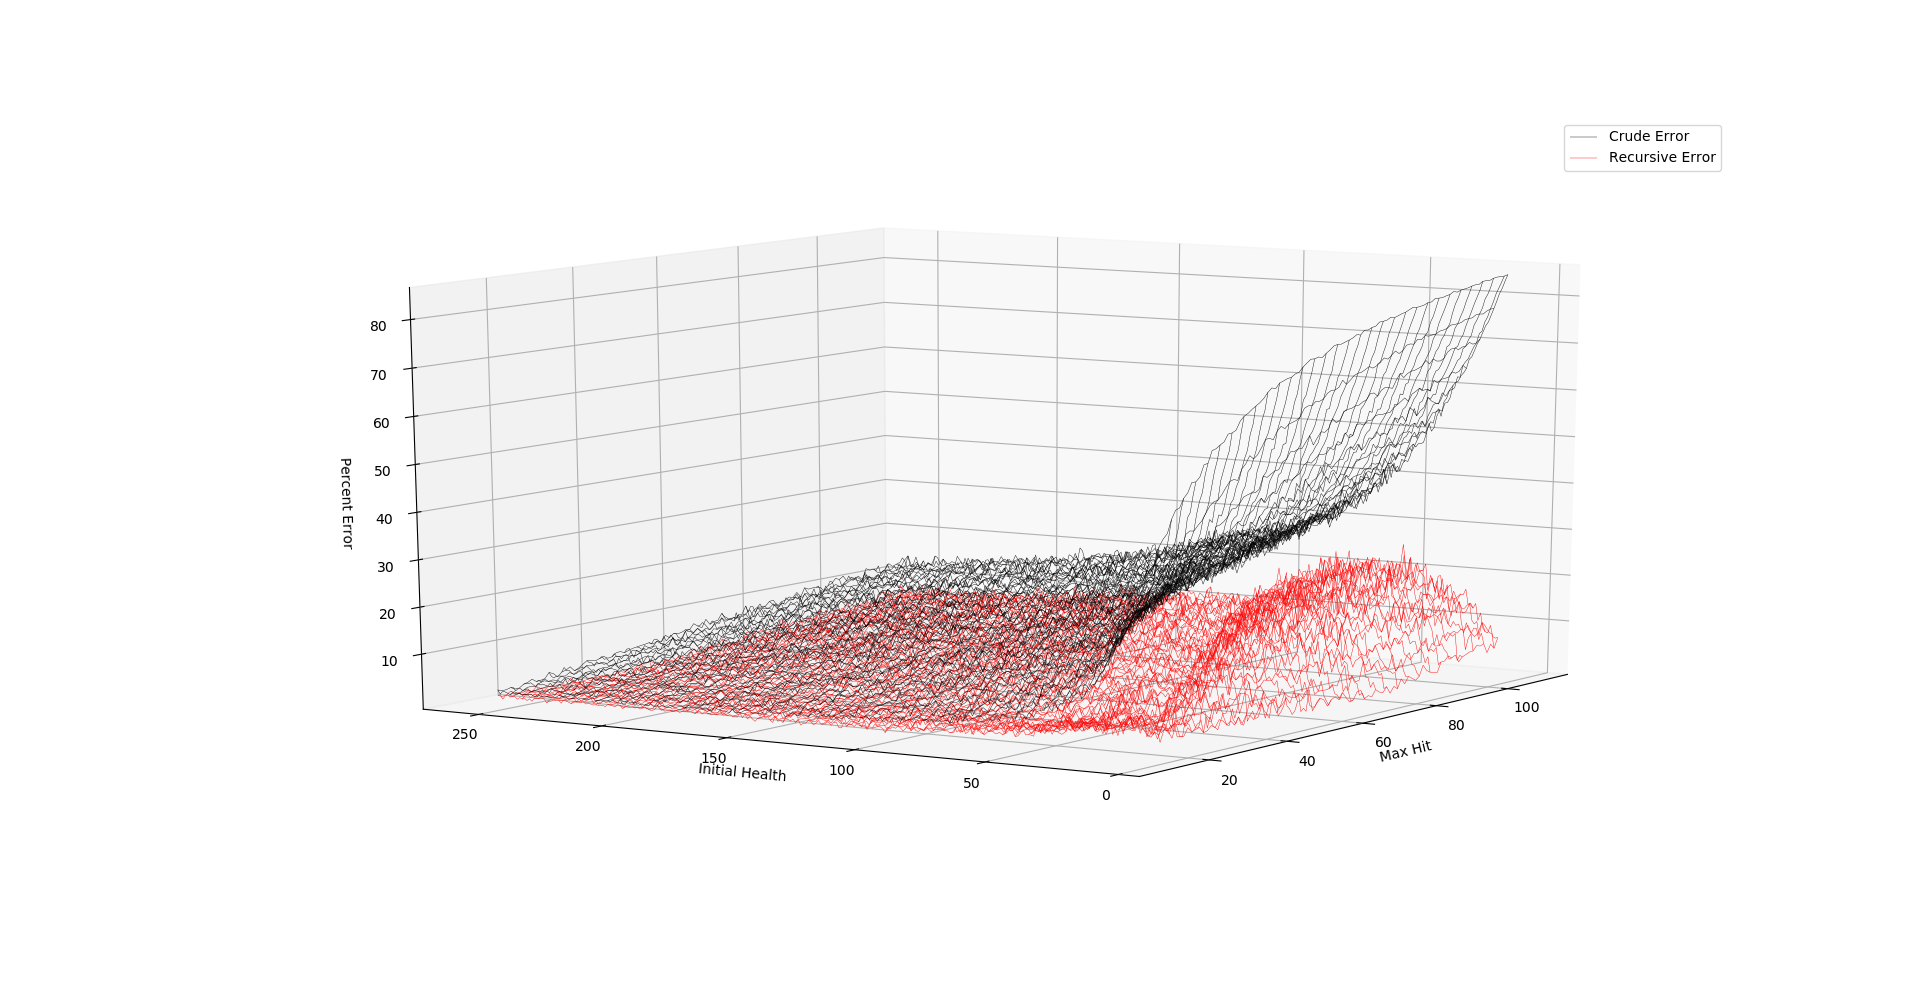
\includegraphics[width=\linewidth]{img/h2k_e2.png}
						\caption{Error from Simulation}
						% \label{fig:sub2}
					\end{subfigure}
					\caption{A comparison between different models. The crude model does not consider any overkill influence and therefore considers Eq.~\ref{eq:h_crude} to hold everywhere. The recursive model is that described in Eq.~\ref{eq:recursive_h} which best accounts for overkill. Finally the simulation model is calculated by simulating many fights and averaging the results, within the standard error this is the true solution. On the left, the expected turns to kill (specifically number of successful hits) which shows a steep increase as the max hit drops further below the initial health. All three models \textit{appear} quite similar, however this is an artifact of scale. On the right, the percent relative error with respect to the simulations are shown. The noise is evident and occurs due to the difficulty of efficiently simulating the required number of fights (which justifies attempting to get analytic solutions!). In addition, we see that the error is highest for high max hits, and low initial health often reaching over 10\% in this domain. This makes sense since this is where overkill is expected. The recursive method typically has under half the error of the crude method. Furthermore, the error is unbounded in the crude case, whereas the recursive solution has a global maximum.}
					\label{fig:comparison}
				\end{figure}




		\subsection{Experience and Damage Per Second}
			We saw that by inverting the health per attack equation, we could determine the average number of successful attacks required to kill an opponent based on the max hit and starting health. We first need to extend this to number of \textit{total} attacks, which is relatively straight forward. For this accuracy, $a\in[0, 1]$ has to be factored in. For the health per turn, $h(n)$, we simply note that $h(n)\to h(na)$ will appropriately reduce the number of ``effective turns''. Similarly, for turns to kill, $h^{-1}(1)=n\to n/a$ appropriately extends the number of turns expected. So multiplying and dividing easily accounts for accuracy.

			This can further be extended to time to kill by considering the time it takes for each attack. Let $s$ be the attack speed (in attacks per second), then $n/(as)$ is the required time to kill an opponent. While the health at a given time, $t$ is $h(tas)$. This is a good time to note that the error shown in Fig.~(\ref{fig:comparison}) is unchanged since these multiplicative factors cancel out in the relative error calculation.

			Experience is calculated as a multiple, $e$ of the damage done. So if the opponent has $h_0$ health, and they are killed in $n/(as)$ seconds, then the experience per second is,
			\begin{equation}
				\boxed{E=eash_0/n}
			\end{equation}
			noting that $n$ is also a function of $h_0$, so $E$ does \emph{not} increase linearly with $h_0$.

	\section{Nightmare Zone}
		We can now attempt to extend this into an useful application. For practical purposes, the Nightmare Zone (NMZ) is a combat training ground that offers a low intensity, but efficient method of training combat skills. The player enters an arena with several bosses they have previously fought. At any given time, four (randomly chosen - with replacement) are in combat with the player. Before beginning, the player can decide a minimum of five bosses they would like to re-fight.

		\begin{figure}
			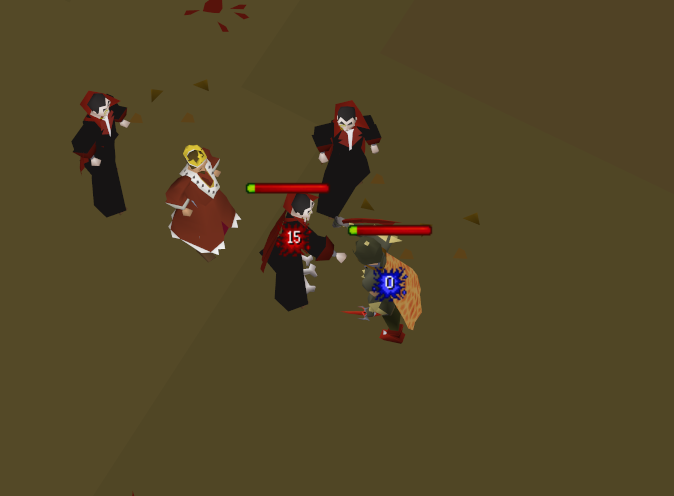
\includegraphics[width=\linewidth]{img/NMZ.png}
			\caption{A player (bottom-right) fighting against four bosses in the NMZ. Three of the bosses at this time happened to be the same, however each bosses is expected to occur with equal probability.}
			\label{fig:nmz}
		\end{figure}

		This can be seen as a first a check, and second an optimization problem (to maximize experience). At this point we have calculated the experience per hour in terms of: accuracy, max hit, initial opponent health, and attack speed. The accuracy and max hit are involved yet straightforward calculations, while the other parameters are generally in a database. We have only made two assumptions so far, no health regeneration, and constant combat, along with 1 approximation in the turns to kill formula. 1 health is regenerated every minute the opponent is under their maximum health. Thus, kills under on minute shouldn't be affected by this, while kills on the order of a few minutes only have a very small influence (since the duration of the fight typically implies high health). The lower the initial health of the opponent, the lower the impact of health regeneration.

		\begin{figure}
			
\includegraphics[width=\linewidth]{img/Details.png}
			\caption{The main setup used for validation. Certain tests used Dharok's greataxe as the weapon, instead of the dragon scimitar (shown).}
			\label{fig:setup}
		\end{figure}

		\subsection{Validation}
			To increase the probability that the player will remain in combat, only opponents who occupy a single tile will be used (that way more can stack up on the player, and they are more likely to retaliate against someone). For the sake of accuracy and reducing human error, no prayers, or special attack will be used. Additionally, tank gear, and absorption potions will be used to minimize the influence of sustaining the player's health. \href{https://runelite.net/}{Runelite}'s built-in experience rate tracker will be used to collect data.
			% 1x1 opponents

			\subsubsection{Potions \& Dharok}
				Dharok is a set of equipment which provides increased damage based on the health missing from the player. Since health recovers at a rate of one health per minute, and the boosted level from potions decreases one level per minute, these introduce time-dependent experience rates. Thankfully, the treatment is relatively simple. Let $a = a(t)$, and $m = m(t)$. At each boosted state, we can calculate the expected experience rate, and average over the boosted states:
				\begin{align}
					\boxed{\langle E \rangle = \frac{1}{N}\sum_{i=0}^{N} E(a(t_i), m(t_i))}
				\end{align}
				For example, if the player re-drinks a potion after $N=10$ levels have dropped, then the above determines the average experience. Things are a little bit more complex when both potions and Dharok are used since the timings might not line up, but for large simulations that detail gets averaged out.

			\begin{tabularx}{\textwidth}{X|XXXXXX|}
				\textbf{Settings} & \textbf{Crude} & \textbf{Recursive} & \textbf{Simulation} & \textbf{Bitterko...} & \textbf{Actual}\\\hline\hline\\
				\noindent\parbox[c]{1.5\hsize}{Easy\\No Potions\\D Scim.\\1.47h} &
				66.9k (\textcolor{red}{17.3\%}) &  58.9k (\textcolor{green}{3.10\%}) & 58.3k (\textcolor{green}{2.00\%}) & 65.8k (\textcolor{red}{15.21\%}) & 57.1k \\\\\hline\\

				\noindent\parbox[c]{1.5\hsize}{Hard\\No Potions\\D Scim.\\1.56h} &
				66.1k (\textcolor{red}{5.01\%}) &  63.3k (\textcolor{green}{0.50\%}) & 63.0k (\textcolor{green}{0.07\%}) & 65.8k (\textcolor{red}{4.42\%}) & 63.0k \\\\\hline\\

				\noindent\parbox[c]{1.5\hsize}{Easy\\Potions\\D Scim.\\1.43h} &
				66.9k (23.4\%) &  13k (23.4\%) & 13k (23.4\%) &13k (23.4\%) & 13k \\\\\hline\\

				\noindent\parbox[c]{1.5\hsize}{Hard\\Potions\\D Scim.\\1.43h} &
				66.9k (23.4\%) &  13k (23.4\%) & 13k (23.4\%) &13k (23.4\%) & 13k \\\\\hline\\


				\noindent\parbox[c]{1.5\hsize}{Easy\\Potions\\Dharok.\\1.43h} &
				66.9k (23.4\%) &  13k (23.4\%) & 13k (23.4\%) &13k (23.4\%) & 13k \\\\\hline\\

				\noindent\parbox[c]{1.5\hsize}{Hard\\Potions\\Dharok.\\1.43h} &
				66.9k (23.4\%) &  13k (23.4\%) & 13k (23.4\%) &13k (23.4\%) & 13k \\\\\hline\hline
				\caption{
					Experience per hour calculated according to different methods, for a few setups (percent errors from the actual gameplay are given in parenthesis). Easy or Hard corresponds to the boss difficulty which only increases their offensive capability and their health, which offers a good probe for the models, and this only modifies one relevant parameter. Two weapons were tested the dragon scimitar (a standard training weapon), and the Dharok's greataxe which has a health (and therefore time) dependent bonus. Finally, the gameplay time for the actual measurement is also stated. Since the largest (still small) source of errors in all models (constant combat, and health sustaining (absorptions potions)) negatively impact experience rates, we expect the models to be tight upper bounds on the actual gameplay experience. A relatively generous error on the actual experience is 1k.
				}
			\end{tabularx}

			% \begin{table}[]
			% 	\centering

			% 	\begin{tabular}{llccccc}
			% 		\textbf{Settings} & \textbf{Crude} & \textbf{Recursive} & \textbf{Bitterkoekje} & \textbf{Actual}\\\hline
			% 		No Potions\\No Prayer\\D Scim.\\ & 66.9k (23.4\%) &  13k (23.4\%) & 13k (23.4\%) & 13k\\\\\\\\
			% 	\end{tabular}
			% 	\begin{tabular}{lcccccc}
			% 		\textbf{Settings} & \textbf{Opponent} & \textbf{Crude} & \textbf{Recursive} & \textbf{Bitterkoekje} & \textbf{Actual}\\\hline
			% 		\multirow{2}{2cm}{Potions\\No Prayer\\D Scim.\\}
			% 		& King Roald & 1& 2& 3& 4\\
			% 		& King Roald & 1& 2& 3& 4\\
			% 		& King Roald & 1& 2& 3& 4\\
			% 		& King Roald & 1& 2& 3& 4\\
			% 		& King Roald & 1& 2& 3& 4\\
			% 		& Overall & 1& 2& 3& 4\\
			% 	\end{tabular}
			% 	\begin{tabular}{lcccccc}
			% 		\textbf{Settings} & \textbf{Opponent} & \textbf{Crude} & \textbf{Recursive} & \textbf{Djon} & \textbf{Actual}\\\hline
			% 		\multirow{2}{2cm}{Potions\\No Prayer\\Dharok.\\}
			% 		& King Roald & 1& 2& 3& 4\\
			% 		& King Roald & 1& 2& 3& 4\\
			% 		& King Roald & 1& 2& 3& 4\\
			% 		& King Roald & 1& 2& 3& 4\\
			% 		& King Roald & 1& 2& 3& 4\\
			% 		& Overall & 1& 2& 3& 4\\
			% 	\end{tabular}
			% 	\caption{}
			% \end{table}

		\subsection{Optimization}
			We can consider the player's choice, along with there equipment as parameters to an optimization problem. Furthermore, more practically, this can be considered as an equipment cost versus experience rate optimization.

	\section{Improvements}
		Health regeneration. Analytic solution? Constant Combat. Health Sustainability. The last two shouldn't impact rankings since they are multiplicative and independent of the calculation method.














		\newpage
		\begin{appendices}
			Here we will attempt to derive a more useful form of Eq.~\ref{eq:recur}. We will start with a slightly simpler relation,
			\begin{align}
				h_{n+1} &= h_n^2 + h_n.
			\end{align}
			We note that in general, this will be an expansion in terms of $h_0$,
			\begin{align}
				h_n = \sum_{i=1}^m a_i h_0^i.
			\end{align}
			Our goal then, is to determine the set of coefficients ${a_i}$. These coefficients implicitly depend on $n$. Our next iteration will look like,
			\begin{align}\label{eq:sum_n+1th_term}
				h_{n+1} = \left(\sum_{i=1}^m a_i h_0^i\right)^2 + \sum_{i=1}^m a_i h_0^i.
			\end{align}
			The squared term is actually very messy to deal with, requires the use of the Multinomial Theorem which (for the specific case $p=2$) states,
			\begin{align}
				\left(\sum_{i=1}^m x_i\right)^2 = 2\sum_{\{k_m\}=2} \prod_{t=1}^m \frac{x_t^{k_t}}{k_t!},
			\end{align}
			where $\{k_m\}=2$ denotes the sets of $m$ integers which add to two. For $m=4$ one example might look like: $(1, 0, 0, 1)$. For those of you familiar with this, these sets arise from integer partitioning, but we won't go over how these are generated, but just know there are algorithms for generating them. We will drop the $=2$ portion for brevity. Our form can be obtained with the transformation $x_i\to a_ih_0^i$,
			\begin{align}
				\left(\sum_{i=1}^m a_ih_0^i\right)^2 &= 2\sum_{\{k_m\}} \prod_{t=1}^m \frac{a_t^{k_t} h_0^{tk_t}}{k_t!} \\
				&= 2\sum_{\{k_m\}} \prod_{t=1}^m \frac{a_t^{k_t}}{k_t!} h_0^{\sum_{t=1}^m tk_t}.
			\end{align}
			Now let's return to the general n'th term (Eq.~\ref{eq:sum_n+1th_term}),
			\begin{align}
				h_n = 2\sum_{\{k_m\}} \prod_{t=1}^m \frac{a_t^{k_t}}{k_t!} h_0^{\sum_{t=1}^m tk_t} + \sum_{i=1}^m a_i h_0^i.
			\end{align}
			As-is, these cannot be combined. To handle this, we impose an ordering on $\{k_m\}$ so they they are given in increasing values of $\sum tk_t$, we will denote this as $\{k_m\}_i^{L}\uparrow$, where $L$ indicates the sum's value for the current set, and $i$ is the index of the current set. Now,
			\begin{align}
				h_n = 2\sum_{\{k_m\}_i^L\uparrow} \prod_{t=1}^m \frac{a_t^{k_t}}{k_t!} h_0^{L_m} + \sum_{i=1}^m a_i h_0^i.
			\end{align}
			Our only hope of combining these terms is to match up the powers. The good news is that now each term on the left, and right correspond to a single power.
			\begin{align}
				h_n = 2\sum_{\{k_m\}_i^L\uparrow} \left(\prod_{t=1}^m \frac{a_t^{k_t}}{k_t!} + a_i \right) h_0^{L_m},
			\end{align}
			Now, we should start from the bottom ($n=0$) and see if we can build up. For $n=0$, $h_{1}=h_0^2+h_0$. So the coefficients are $\{a\}^1 = (1, 1, 0, 0, 0, ...)$, where the zero padding accounts for the fact that the powers on the linear sum are less than the powers on the quadratic sum.

			We can read off the coefficient is we sort-of invert the sum notation. Let's instead sum across $i$.
			\begin{align}
				h_n = 2\sum_{i} \left(\prod_{\{k_t\}_i}^m \frac{a_t^{k_t}}{k_t!} + a_i \right) h_0^{L_i}.
			\end{align}
			Now the coefficient for the $L_i$'th power for the next iteration is
			\begin{align}
				a_{L_i} = 2\left(\prod_{\{k_t\}_i}^m \frac{a_t^{k_t}}{k_t!} + a_i \right).
			\end{align}
			This actually works out really well since the coefficients for our original problem simply get multiplied by $\gamma$! Let's make another simplification by letting $k_t$ be represented by a vector, $\vec k$ and constructing respective operations,
			\begin{align}
				a_{i, n+1} = 2 \frac{\boldsymbol{a}_n^\boldsymbol{k_i}}{\boldsymbol{k_i}!} + 2a_{i, n}.
			\end{align}
			Here a vector to the power of a vector is the product of the element-wise powers, and the factorial of a vector is the product of the element-wise factorials.
		\end{appendices}


\end{document}
